\documentclass{article}
\usepackage[swedish]{babel}
\usepackage[utf8]{inputenc}
\usepackage[a4paper, total={17cm, 21cm}]{geometry}
\usepackage{graphicx}
\usepackage[backend=bibtex]{biblatex}
\addbibresource{uni.bib}
\title{Mjukvaruutveckling av visualiseringssystem\\
\Large {Projektplan}
}

\author{Rohullah Khorami \& Fredrik Kortetjärvi }


\begin{document}

\maketitle
\newpage
\tableofcontents
\newpage

\section{Introduktion}Det är ett stort behov av ett visualiseringssystem kopplat mot fastighetssystemet KNX. Att driftsätta och testa av
en större fastighet är mycket tidskrävande och risken för att missa någon avvikelse är stor. 
För systemet finns en färdig drivrutin för Windows och .NET, med funktioner för att koppla upp mot systemet.
Applikationen ska således utvecklas mot .NET i valfritt passande språk.

\section{Syfte}Den tilltänkta applikationen kommer kvalitetssäkra testning och minska tidsåtgången att testa systemet på olika fastigheter avsevärt. Syftet är då att ta fram en applikation från grunden som kopplar upp mot
fastighetssystemet (via befintlig drivrutin) och lyssnar av trafiken för att logga och visa upp denna grafiskt.

\section{Metod}
Applikationen behöver vara dynamisk, dvs. kunna laddas med strukturerad data (t.ex. från xml eller csv) för att
med denna data automatiskt generera visning och kontroller i applikationen enligt uppsatta regler. En skiss kommer görs till applikationen sen programmet kommer delas i små delar för att kunna jobba mer effektivera och kunna strukturera hela koden. Vi komma ha ett möte varannan vecka med företaget och ett möte per vecka med handledaren för att kunna hålla processen på rätt bana och för att undvika onödiga arbete. \newline
\subsection{Språk \& verktyg}
Applikationen kommer vara i C\# för att kunna koppla applikationen med .NET drivrutin. Det behöver bara vara i Windows då företaget bara använder Windows. Andra föredel med C\# är att graphical user interface(GUI) delen är "inbyggd". Det går att använda andra språk också t.ex C eller C++ och dessa har fördelar som har en snabb exekveringstid och är lättviktigt språk. C och C++ är cross-plattform program fast C \& C++ har separata GUI bibliotek därför det är lämplig att använda C\# för programmera applikationen.Visual studio 2019 och C\# kommer används för att programmera applikationen för att det är enklare att lansera koden och har bra verktyg att debugger och integrerar med dll filen.\cite{CPROG}\newline 
\subsection{Person \& Ekonomi}
Sundas Munir kommer vara vår handledare genom att hon hjälper med att skriva rapporten och diskutera kring problem. Marcus Karlsson är vår kontakt person på Teknisk Byrån som kommer ge oss mer information och resurser. Projekt processen har inte något kostnad för att företaget kommer fixa visa hårdvaror för att testa applikationen i slutet. Projektet kommer görs i Högskolan eller hemma då behöver vi inte träffa företaget då finns inget reskostnad heller. \newline
\subsection{Materiel}
Drivrutiner fås från företaget som kommer kopplas till KNX systemet som låter applikationen kommunicera med KNX kompatibla produkter som kommer testas. Företaget har skapat en dokumentation om hur drivrutinen kommer kommunicera med koden. Hårdvara kommer komma från tekniska byrån som kommer vara en del av test fasen. När vi ska testa applikationen då använder vi några filer som vi har fått från företaget.
\subsection{Resultatutvärdering}
Programmet kommer testas med hjälp av hårdvara från företaget 
och kommer även testas av företaget själva för att applicera produkten i verkligheten. Efter testet kommer respons från företaget som avgör hur färdig produkten är samt hur effektivt och användbar programmet är i dags läget. Felen som kan kommas komma upp är att resultatet av programmet inte är användbart eller oläsligt. Efter responsen kommer dra slutsats hur mycket som måste göras för att bli färdiga med produkten.
Förväntningsresulatet kommer ser ut som figur \ref{fig:GUI} där en fil laddas upp i applikationen sen programmet visualisera det vill säga programmet delar data i små delar. På högra delen av applikationen går det att sätta värde och sen med hjälp av "Check" knappen kommer det visa respons i vänstra nedre delen, i text format.\newline
\begin{figure}
    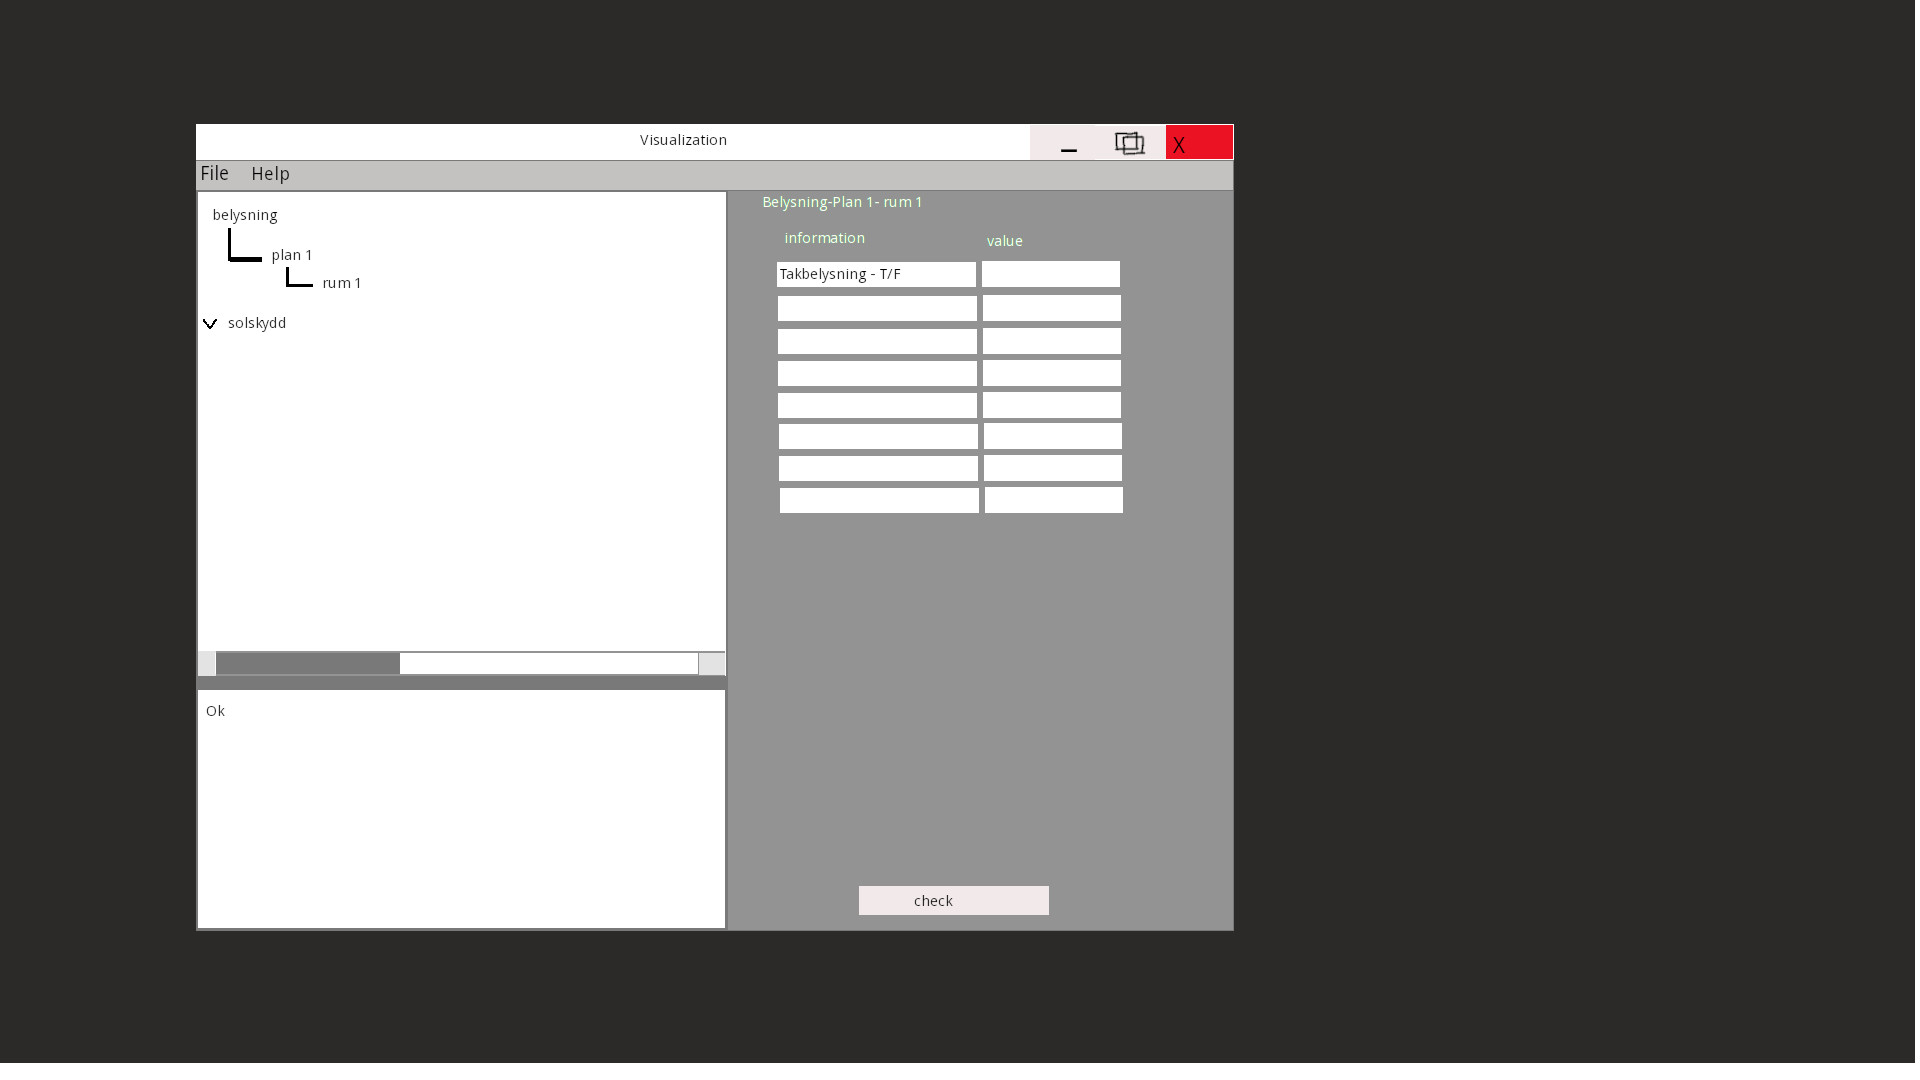
\includegraphics[width=\linewidth]{../SourceFiles/Visualization.jpg}
    \caption{Graphical user interface.}
    \label{fig:GUI}
\end{figure}
\subsection{UtExpo}
Under UtExpo kommer mjukvaran och relation mellan mjukvaran och hårdvaror visas. Det innebär att hur hårdvaror kommer kommunicera med applikationen och även koden kan presenteras om det behövs.\newline
\newpage
\section{Tidsplan} 
\begin{table}[h!]

    \begin{tabular}{|c|c|}
        \hline
        \textbf {Uppgift} & \textbf{datum}  \\
        \hline
        Planering av GUI delen, hur applikationen kommer se ut grafiskt & 25-01-2021 -- 31-01-2021 \\
        \hline
        Delar applikationen i små delar som kan arbetas separat & 01-02-2021 -- 02-01-2021\\
        \hline
        Själva programmering processen & 03-02-2021 -- 01-04-2021\\
        \hline
        Halvtids seminarie färdigt & 05-03-2021 -- 12-03-2021\\
        \hline
        På börja presentation  & 10-05-2021 -- 15-05-2021 \\
        \hline
        Rapport skrivning & 15-02-20201 -- 14-05-2021\\
        \hline
        Förberedelse till UtExpo(om det blir av) & UTExpo en vecka innan \\
        \hline
    \end{tabular}
\end{table}
\newpage
\printbibliography
\end{document}

